L'analyse morphologique entre les graphes de flot de contrôles de plusieurs binaires peut également être utilisée pour détecter l'utilisation de fonctionnalités similaires entre ces programmes et faire correspondre précisément des morceaux de code assembleur de l'un et de l'autre.

Dans ce chapitre nous présentons des travaux réalisés en ce sens sur un logiciel malveillant, Waledac, qui utilise une bibliothèque connue de chiffrement, OpenSSL.
Ces travaux ont fait l'objet d'une communication orale à REcon en 2012 \cite{REAT12} et d'une publication à Malware \cite{mal12}.

% \section{Problème : accélérer l'analyse}
\section{Contexte d'analyse de code}
L'analyse manuelle de code binaires inconnus est à la base de tout travail sur la détection de logiciels malveillants.
L'analyste cherche d'une part à déterminer et comprendre l'ensemble du code du programme afin d'en connaître les fonctionnalités
et le classer comme logiciel malveillant ou légitime.
D'autre part, s'il s'agit d'un logiciel malveillant, il cherche à établir une signature du binaire permettant de détecter sa présence sur une machine infectée et, éventuellement, de le supprimer.
L'analyse se fait à l'aide de différents outils, dont un désassembleur interactif tel IDA \cite{IDA} ou Radare \cite{radare} pour l'analyse statique et d'un outil pour l'analyse dynamique comme un débogueur, un émulateur ou un logiciel d'instrumentation.

Les logiciels analysés ne présentent en général pas d'informations de compilation permettant d'identifier les bibliothèques logicielles utilisées ni leur version. Nous cherchons à automatiser la recherche de bibliothèques connues dans un logiciel à analyser et à marquer son emplacement dans un désassembleur interactif (IDA) afin d'éviter l'analyse inutile de code documenté et accélérer l'analyse manuelle.

\subsection{Waledac et OpenSSL}
Waledac \cite{CRFLSGBA10}, apparu en 2008, est un botnet, c'est à dire un programme malveillant transformant les machines infectées en esclaves (ou \emph{zombies}) recevant des ordres d'un serveur de commande et de contrôle (C\&C).
Les machines esclaves communiquent entre elles sous la forme d'un réseau pair à pair et la charge finale principale du réseau est l'envoi de courrier électronique non sollicité (\emph{spam}).
Il s'agit d'un programme dont les fonctionnalités étaient déjà bien connues et documentées lorsque l'on a commencé à travailler dessus. Notre objectif était alors de voir s'il était possible d'automatiser une partie de l'analyse, sachant qu'on serait capables de vérifier nos résultats à l'aide d'analyses manuelles existantes.

Afin de savoir quelles méthodes de chiffrement il utilise, nous avons cherché des chaînes de caractères dans le binaire correspondant à quelques bibliothèques standard à l'aide du l'outil \emph{strings}.
Par chance il était facile de trouver qu'il utilise la version 0.9.8e de OpenSSL:
\begin{verbatim}
$ strings "Waledac v48 unpacked.exe" | grep OpenSSL
   EC part of OpenSSL 0.9.8e 23 Feb 2007
   ECDSA part of OpenSSL 0.9.8e 23 Feb 2007
\end{verbatim}

OpenSSL \cite{openssl} est une bibliothèque libre et documentée, elle ne devrait nécessiter une analyse de son code binaire ici inclut dans Waledac. Nous voulons également connaître précisément les fonctions utilisées ainsi que parties de code communes.

\section{Analyse morphologique}
% \subsection{Trouver des sites communs}
La technique d'analyse morphologique détaillée aux deux chapitres précédents a été directement utilisée : on détermine les graphes de flot de contrôle de chacun des deux binaires, on leur applique des réductions puis on les découpe en sites.
On cherche ensuite des sites communs entre les Waledac et OpenSSL.

\paragraph{Taille des graphes de flot.}
Les binaires sur lesquels nous avons travaillé ont des graphes de flot de contrôle initiaux allant jusqu'à quelques centaines de milliers de sommets avant réduction et environ quinze mille sommets après réduction. Nous avons initialement trouvé 53 sites communs entre la version 0.9.8x de OpenSSL et Waledac.
Nous avions initialement pris la version 0.9.8x, la version à jour d'OpenSSL, les versions antérieures n'étaient pas disponibles sous forme binaire pour Windows et nécessitaient d'être compilées.

\begin{figure}[h]
\begin{tabular}{|l|l|l|l|}
\hline
 Binaire & Taille du GFC & Taille du GFC réduit & Nombre de sites de taille 24 	\\
\hline
 Waledac &  38236 & 14626 & 11141					  	\\
\hline
 OpenSSL 0.9.8x  & 174754 & 28313 & 22171				  	\\
\hline
\end{tabular}
\end{figure}

\paragraph{Influence des options de compilation.}
Nous avons ensuite compilé la version 0.9.8e en utilisant différentes options de compilation utilisées avec le compilateur pour Windows Visual Studio.
Nous avons pu remarquer que l'option donnant le plus sites en commun était celle compilée pour optimiser la taille du binaire. Le tableau suivant donne le nombre de sous-sites communs entre Waledac et chacune des versions de OpenSSL.

\begin{figure}[h]
\begin{tabular}{|l|l|l|}
 \hline
Version & Remarque & Sites communs \\
 \hline
0.9.8x & Version de mai 2012 & 53 \\
0.9.8e & Optimise les performances temporelles (/0x /02) & 53 \\
0.9.8e & Optimise la taille du fichier (/01) & 1264 \\
 \hline
\end{tabular}
\end{figure}

\subsection{Correspondance fine entre instructions}
Dans un second temps nous voulons être capables de marquer, dans le désassembleur, les instructions ainsi que les fonctions assembleur qui ont été reconnues.
Nous avons utilisé les techniques précédentes pour qu'en plus de retourner une correspondance entre un site du graphe de motif P et un site du graphe de test T, nous ayons aussi l'information précise donnant la correspondance entre un sommet du sous-site de motif et un sommet du sous-site de test. Tous les algorithmes présentés au chapitre précédent fournissent cette information.

Nous supposons donc que l'on dispose de la fonction \emph{match} qui, à partir d'un sous-site $S_P$ de $P$ et d'un sous-site $S_T$ de $T$, renvoie une liste de couples de correspondance entre un sommet de $S_P$ et un sommet de $S_T$. Dans le cas où les deux sous-sites ne correspondent pas, elle renvoie $\emptyset$.

Comme décrit dans l'algorithme \ref{algo:correspondance_fine}, nous considérons que plus la taille des sous-sites correspondants est grande, plus la correspondance entre les sommets sera précise.
Nous cherchons en premier lieu le plus grand sous-site que l'on retrouve dans P et T et nous associons tous les sommets de P et de T  correspondants dans ce sous-site. Nous récupérons l'ensemble des sous-sites d'une certaine taille de $P$ et $T$ à l'aide de l'algorithme \ref{algo:generation_site_largeur} du chapitre précédent.
Puis nous continuons avec un sous-site commun plus petit, en associant les sommets qui n'ont pas encore été associés, et ainsi de suite jusqu'à atteindre la taille initiale des sites choisis pour la détection, soit W. 

\begin{figure}[h]
\begin{algorithm}[H]
\DontPrintSemicolon
\caption{Association des sommets de deux graphes de flot de contrôle}
\SetAlgoLined
\KwIn{Deux graphes de flot, P et T de taille respective $n_P$ et $n_T$, la taille minimale des sites recherchés, W}
\KwResult{Une liste de correspondances sommet à sommet entre P et T}
\SetKwProg{Fn}{}{}{}
\SetKwFunction{FRecurs}{association}
\Fn(
% \tcc*[h]{C : matrice des associations possibles, i : numéro du prochain sommet de P à associer, F : liste des couples d'associations déjà faites}
){\FRecurs{P, $n_P$, T, $n_T$, W}}{
$L\leftarrow \emptyset$\\
$A_P, A_T \leftarrow (\emptyset, \emptyset)$ \tcc*{ensembles des sites de T et P associés}
$m\leftarrow min(n_P, n_T)$\\
\tcc{On extrait tous les sites :}
\For {$W \leq i\leq m$} {
  $S_{P, i}\leftarrow sites(P, i)$\\
  $S_{T, i}\leftarrow sites(T, i)$
}
$k\leftarrow m$\\
\While{$k\geq W$}{
\For{$S_P\in S_{P, k}$}
{
  \For{$S_T\in S_{T, k}$}
  {
    \tcc{On place dans C les couples de sommets correspondants :}
    $C\leftarrow match(S_P, S_T)$ 
    \For{$(s_P, s_T)\in C$}{
      \If{$s_P\notin A_P$ et $s_T\notin A_T$}{
	$L\leftarrow L\cup \{(s_P, s_T)\}$\\
	$A_P\leftarrow A_P\cup \{s_P\}$\\
	$A_T\leftarrow A_T\cup \{s_T\}$\\
      }
    }
  }
}
$k\leftarrow k-1$
}
\Return{L}
}
\label{algo:correspondance_fine}
\end{algorithm}
\end{figure}

\subsection{Implémentation et résultats}
\paragraph{Correspondance entre sommets.}
La fonction \emph{match} donnant les correspondances a été implémentée pour une variante de l'algorithme d'Ullmann et de l'algorithme par parcours présentés au chapitre précédent, variantes adaptées à la comparaison de sites de mêmes taille.
Elle a également été implémentée dans la version d'origine du détecteur, fonctionnant par automates d'arbres.
Nous avons ajouté, dans le détecteur, une possibilité d'export de ces correspondances.

\paragraph{Greffon IDA.}
Un greffon (ou \emph{plugin}) a été développé pour le désassembleur interactif IDA, permettant, lorsque que deux instances du désassembleur sont lancées, chacune analysant un des deux programmes comparés, d'aligner le code comparé selon les correspondances trouvées au préalable par analyse morphologique.
Le greffon surligne les instructions ayant trouvé un correspondant dans l'autre graphe de flot et donne également la correspondance entre les fonctions assembleur du premier programme et du second.

\paragraph{Exemple avec Waledac et OpenSSL.}
La figure \ref{fig:plugin_subroutines} montre un extrait de la page de correspondances entre les fonctions assembleurs identifiées par IDA entre la DLL principale d'OpenSSL (\emph{libeay32-098e.dll}) et Waledac (\emph{Waledac48.int}). La première colonne indique les adresses des instructions d'OpenSSL correspondant aux instructions présentes aux adresses de Waledac à la troisième colonne. Les deuxième et quatrième colonnes donnent le nom des fonctions assembleur auxquelles ces instructions appartiennent.
OpenSSL ayant été compilé avec des options de débogage, le nom des fonctions est retrouvé par IDA, ce qui n'est pas le cas pour Waledac.
Il est à noter que, puisqu'on a effectué des réductions avant de lancer la comparaison, la plupart des instructions, dont les instructions séquentielles, ne sont pas comparées : ce sont principalement les instructions modifiant le flot de contrôle qui ont été considérées.

% \begin{figure}[h]
% \begin{center}
%  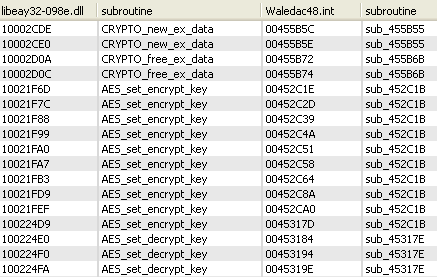
\includegraphics[width=0.8\textwidth]{supports/libs/WalSSLIDA2.png}
% \end{center}
% \caption{Fonctions correspondantes entre OpenSSL à gauche et Waledac à droite}
% \label{fig:plugin_subroutines}
% \end{figure}

\begin{figure}[h]
\begin{center}
\begin{tabular}{|l|l|l|l|}
\hline
\multicolumn{2}{|c|}{OpenSSL (libeay32-098e.dll)} & \multicolumn{2}{c|}{Waledac (Waledac48.int)} \\
\hline
Adresse & Fonction & Adresse & Fonction \\
\hline
 10002CDE & CRYPTO\_new\_ex\_data & 00455B5C & sub\_455B55 \\
 10002CD0 & CRYPTO\_new\_ex\_data & 00455B5E & sub\_455B55 \\
 10002D0A & CRYPTO\_new\_ex\_data & 00455B72 & sub\_455B55 \\
 10002D0C & CRYPTO\_new\_ex\_data & 00455B74 & sub\_455B55 \\
\hline
 10021F6D & AES\_set\_encrypt\_key & 00452C1E & sub\_452C1B \\
 10021F7C & AES\_set\_encrypt\_key & 00452C2D & sub\_452C1B \\
 10021F88 & AES\_set\_encrypt\_key & 00452C39 & sub\_452C1B \\
 10021F99 & AES\_set\_encrypt\_key & 00452C4A & sub\_452C1B \\
 10021FA0 & AES\_set\_encrypt\_key & 00452C51 & sub\_452C1B \\
 10021FA7 & AES\_set\_encrypt\_key & 00452C58 & sub\_452C1B \\
 10021FB3 & AES\_set\_encrypt\_key & 00452C64 & sub\_452C1B \\
 10021FD9 & AES\_set\_encrypt\_key & 00452C8A & sub\_452C1B \\
 10021FEF & AES\_set\_encrypt\_key & 00452CA0 & sub\_452C1B \\
 100224D9 & AES\_set\_encrypt\_key & 0045317D & sub\_452C1B \\
\hline
 100224E0 & AES\_set\_decrypt\_key & 00453184 & sub\_45317E \\
 100224F0 & AES\_set\_decrypt\_key & 00453194 & sub\_45317E \\
 100224FA & AES\_set\_decrypt\_key & 0045319E & sub\_45317E \\
\hline
\end{tabular}
\end{center}
\caption{Fonctions correspondantes entre OpenSSL et Waledac}
\label{fig:plugin_subroutines}
\end{figure}


Nous avons ensuite vérifié, dans IDA grâce à la fonction d'alignement de code du greffon, que le code des instructions correspondantes était bien suffisamment similaire pour valider la méthode.
Une telle correspondance est donnée en exemple à la figure \ref{fig:plugin_code_sync} pour la fonction \emph{AES\_set\_encrypt\_key}.
L'image est constituée d'un bout du graphe de flot de contrôle d'OpenSSL à gauche et d'un bout du GFC de Waledac à droite.
Les instructions surlignées en orange et alignées sont celles pour lesquelles on a trouvé une correspondance.

\begin{figure}[h]
\begin{center}
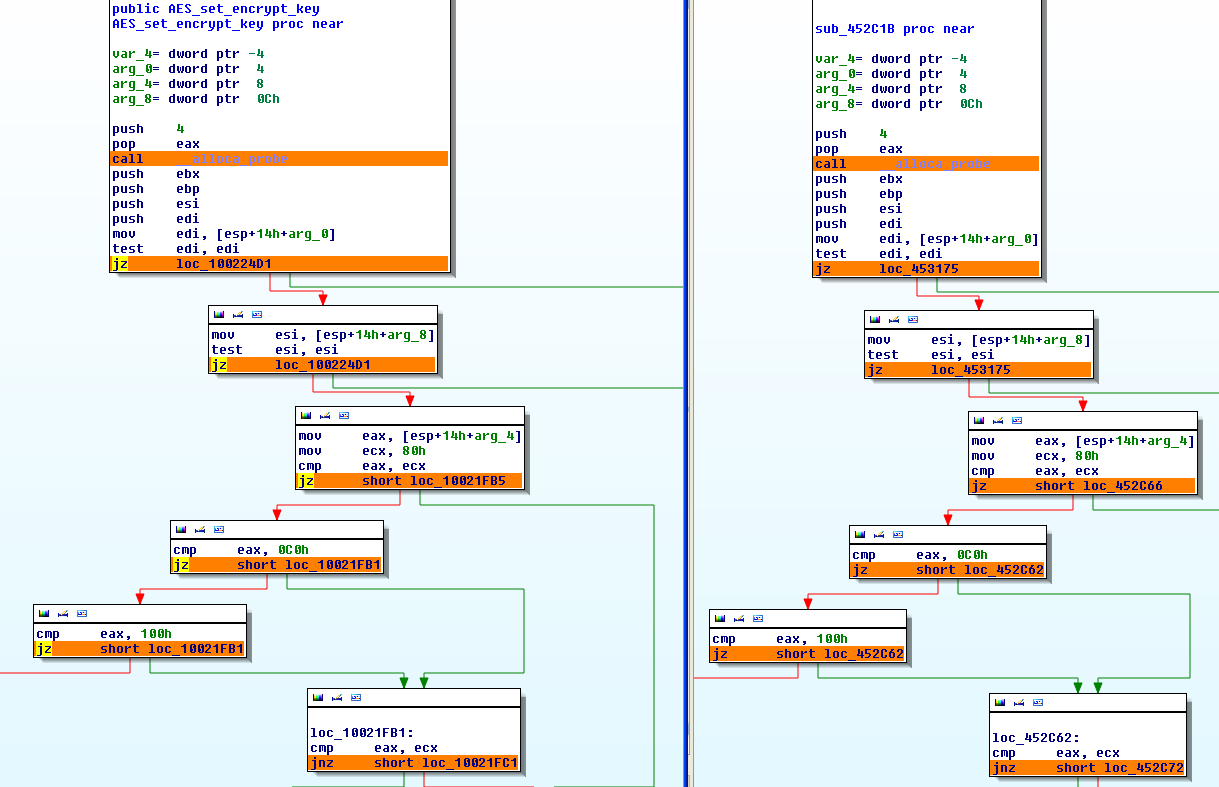
\includegraphics[width=1.0\textwidth]{supports/libs/WalSSLIDAAESgraph.png}
\caption{Capture d'écran d'IDA : Code correspondant entre OpenSSL à gauche et Waledac à droite} 
\label{fig:plugin_code_sync}
\end{center}
\end{figure}

Sur cet exemple nous n'avons pas trouvé de correspondances sommet à sommet qui ne soit pas cohérente mais certaines fonctions n'étaient pas couvertes par suffisamment de sommets pour que l'on soit assurés d'un correspondance.
La figure \ref{fig:tab_fonctionnalites_waledac_openssl} donne un extrait des fonctions d'OpenSSL retrouvées dans Waledac et les fonctionnalités qu'elles fournissent : on y trouve par exemple des méthodes préparant au chiffrement AES, RSA et DSA.

\begin{figure}[h]
\begin{tabular}{|p{9cm}|l|}
\hline
Fonctions 							& Fonctionnalité 			\\
\hline
AES\_set\_encrypt\_key, AES\_set\_decrypt\_key 			& Chiffrement AES 			\\
RSA\_free, DSA\_size, DSA\_new\_method 				& Chiffrement RSA / DSA 		\\
 X509\_PUBKEY\_set, X509\_PUBKEY\_get 				& Certificats X509 			\\
BN\_is\_prime\_fasttest\_ex, BN\_ctx\_new, BN\_mod\_inverse	& Gestion des grands entiers (BN)	\\
CRYPTO\_lock, CRYPTO\_malloc 					& Fonctions génériques d'OpenSSL 	\\
\hline
\end{tabular}
\caption{Fonctions d'OpenSSL retrouvées dans Waledac et fonctionnalités associées}
\label{fig:tab_fonctionnalites_waledac_openssl}
\end{figure}

Il n'est pas surprenant que l'on retrouve ces fonctionnalités puisque Waledac utilise du chiffrement AES et RSA et gères de certifications X509. Notre contribution est que l'on est capable de le montrer sans réellement analyser le code assembleur.

\section{Limites}
On a vu qu'on retrouve certaines fonctions utilisées lors d'un chiffrement AES.
Pourtant nous n'avons retrouvé les fonctions principales, servant à chiffrer et déchiffrer à l'aide de l'algorithme AES.
La raison est que notre approche, par graphes de flot réduits, s'applique très mal aux fonctions de chiffrement qui sont en général très simples du point de vue de leur graphe de flot de contrôle.
Une vue simplifiée du GFC de la fonction \emph{AES\_encrypt} est donnée en figure \ref{fig:AES_encrypt_CFG}.

\begin{figure}[h]
\begin{center}
% \subfigure[AES\_encrypt subroutine]{
% 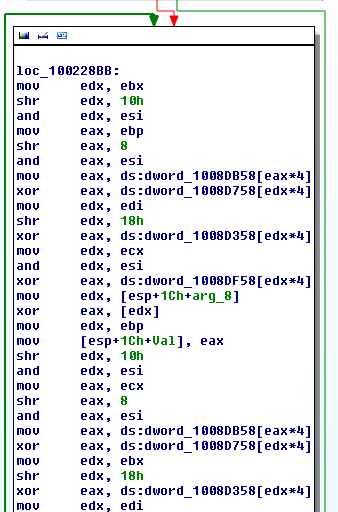
\includegraphics[width=0.4\textwidth]{supports/libs/WalSSLIDAAESencryptnotmatched.png}
% \label{fig:AES_encrypt_IDA}
% }
% \subfigure[]{
\includegraphics[width=0.25\textwidth]{supports/libs/AESsimpleCFG_cropped0.pdf}

% }
\end{center}
\caption{GFC simplifié de la fonction AES\_encrypt}
\label{fig:AES_encrypt_CFG}
\end{figure}

Le GFC réduit est trop petit pour pouvoir être détecté par l'analyse morphologique, qui prend des graphes d'une taille 24 au minimum.
En fait beaucoup d'algorithmes de chiffrement ont cette structure une fois réduits et elle n'est pas non plus spécifique aux algorithmes de chiffrement. De ce fait l'analyse morphologique est inadaptée à la détection de ce genre de fonctions.

\section{Application à Duqu et Stuxnet}
Dans cette section nous présentons nos travaux sur deux programmes malveillants particuliers, \duqu\ et \stux.
Lorsque nous avons commencé ces travaux \stux\ était déjà documenté et détecté, et \duqu\ venait d'être découvert.
Il a rapidement été dit qu'ils étaient semblables et nous avons donc cherché à détecter \duqu\ connaissant \stux.
% Dans un premier temps nous appliquons les travaux présentés au chapitre précédent sur ces exemples \cite{REAT12,mal12}.

\subsection{Duqu et Stuxnet}
% \paragraph{\stux.}
\stux, découvert en juin 2010, est capable de cibler et de reprogrammer des systèmes industriels.
Sans que cela ait été prouvé, il a été avancé qu'il visait le programme nucléaire iranien. 
Symantec \cite{SymantecStux2011} indique que la plupart des systèmes infectés sont en Iran et que la cible pourrait être un système de contrôle de centrifugeuses.
\\

% \paragraph{\duqu.}
\duqu, découvert en premier par Crysys \cite{CrysysDuquStuxnet} en septembre 2011, laboratoire de sécurité et de cryptographie de l'université de Budapest, a directement été détecté comme apparenté à \stux\ parce qu'ils utilisent des techniques d'infection et de propagation similaires.
\duqu\ est un outil offensif utilisé pour le vol d'informations. Symantec \cite{SymantecDuqu2011} a identifié, parmi ses fonctionnalités, des enregistreurs de frappes (\emph{keyloggers}), de l'écran, de l'activité réseau, ainsi que des outils de détection de machines sur le réseau.
Il est maintenu à jour via des serveurs de commande et de contrôle (C\&C) et dispose d'une fonctionnalité d'auto-destruction après, typiquement, 36 jours sans nouvelles du C\&C.

Les attaques semblent réussies puisque le programme malveillant n'a pas été détecté à chaud alors que certaines opérations ont duré plusieurs mois, mais seulement post-mortem. De nombreuses souches de \duqu\ ont été trouvées dans la natures, chacune avec des binaire différents mais similaire. Kaspersky a publié un historique des versions \cite{KaspDuqu10}, la dernière souche détectée date de février 2012, bien après que les première attaques ne soient détectées et documentées.

\paragraph{Analyse des similarités.}
Nous avons effectué une analyse similaire à celle décrite au chapitre précédent pour trouver les similarités entre \stux\ et \duqu\ afin de trouver les parties de \stux\ que l'on retrouve dans \duqu.
Pour ces deux programmes malveillants, nous avons analysé la DLL (bibliothèque logicielle au format Windows, ou \emph{Dynamic Link Library}) principale fois que celle-ci a été déchiffrée.
% Dans les deux cas l'infection est cherche à exploiter une faille de Windows permettant d'installer plusieurs composants qui auront été déchiffrés au préalable.
Nous avons extrait les graphes de flot réduits de \duqu\ et \stux.
Nous avons trouvé 846 sites communs entre \duqu\ et \stux\ : 26.5\% des sites de \duqu\ proviennent de \stux.
Lorsque l'on regarde les sommets correspondants dans les graphes réduits, on s'aperçoit que ces sites contiennent 2215 sommets dans les graphes de flot réduits : 60.3\% des sommets du graphe de flot réduit de \duqu\ correspondent à des sommets  présents dans \stux.

Forts de ces résultats indiquant que \duqu\ et \stux\ partagent beaucoup de code, nous considérons donc qu'un détecteur de programmes malveillant fonctionnant avec la technique d'analyse morphologique connaissant \stux\ serait capable de détecter \duqu.

La principale difficulté qu'aurait à résoudre un détecteur est que le programme provocant l'infection de \duqu\ ne ressemble pas à \stux\ ni à aucun autre programme malveillant connu. Ce n'est que lorsque certains composants de \duqu\ sont déchiffrés et installés que l'on peut le détecter.
Nous détaillerons, dans le chapitre suivant, la méthode d'infection de \duqu\ et le travail nécessaire afin de détecter une attaque.
% Nous avons alors cherché à documenter la méthode d'infection de \duqu\ afin de pouvoir détecter une attaque.


\section{Conclusion}
Nous avons identifié des similarités entre Waledac et une version spécifique d'OpenSSL, nous avons pu reconstruire automatique des correspondances fines afin de déterminer quelles fonctions d'OpenSSL étaient utilisées par Waledac.
L'obstacle principal à une généralisation de cette méthode est qu'elle est sensible aux options de compilation et nécessite de déterminer au préalable les binaires à comparer.
Cette technique n'est pas infaillible puisqu'elle n'est pas adaptée pour détecter certaines structures ou fonctions, telles des fonctions de chiffrement.

Nous avons ensuite développé un greffon pour IDA permettant d'analyser les similarités trouvées afin de permettre à l'analyste de ne pas s'attarder sur du code déjà documenté.
Cette approche, appliquée à \duqu\ et \stux\ nous a permis de mettre en lumière de nombreuses portions de code partagé entre ces deux logiciels malveillants.